\documentclass[tikz,border=10pt]{standalone}
\usepackage{amsmath}
\usepackage{tikz}
\usetikzlibrary{arrows.meta, positioning, calc}

\begin{document}
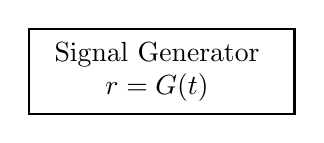
\begin{tikzpicture}[
  block/.style = {draw, thick, minimum height=3em, minimum width=6em, align=center},
  circ/.style  = {draw, circle, thick, minimum size=2.5em, inner sep=0pt},
  arrow/.style = {thick, -{Latex[width=2mm]}},
  node distance=2.5cm and 2.5cm
]

  % Signal Generator box
  \node[block] (siggen) {
    \begin{tabular}{c}
      Signal Generator \\
      $r = G(t)$
    \end{tabular}
  };

\end{tikzpicture}
\end{document}  
